Consider a bivariate normal distribution with $\mu_{1} = 0$, $\mu_{2} = 2$, $\sigma_{11} = 2$, $\sigma_{22} = 1$ and $\rho_{12} = 0.5$.
\begin{enumerate}[label=(\alph*)]
    \item Write out the bivariate normal density.
    For
    \[
        \textbf{x}
        =
        \begin{bNiceArray}{c}
            X_1 \\
            X_2
        \end{bNiceArray},
        \hspace{0.2in}
        \bm{\mu}
        =
        \begin{bNiceArray}{c}
            \mu_1 \\
            \mu_2
        \end{bNiceArray}
        =
        \begin{bNiceArray}{c}
            0 \\
            2
        \end{bNiceArray},
        \hspace{0.2in}
    \]
    \[
        \bm{\Sigma}
        =
        \begin{bNiceArray}{cc}
            \sigma_{11} & \sqrt{\sigma_{11}}\sqrt{\sigma_{22}}\rho_{12} \\
            \sqrt{\sigma_{11}}\sqrt{\sigma_{22}}\rho_{12} & \sigma_{22}
        \end{bNiceArray}
        =
        \begin{bNiceArray}{cc}
            2 & 0.50\sqrt{2} \\
            0.50\sqrt{2} & 1
        \end{bNiceArray}
    \]
    \[
        f(\textbf{x} \big| \bm{\mu},\bm{\Sigma})
        =
        \frac{1}{{(2\pi)}^{p/2}{\left|\bm{\Sigma}\right|}^{1/2}}
        {e}^{\frac{-1}{2}{(\textbf{x} - \bm{\mu})}^{\prime}\bm{\Sigma}(\textbf{x} - \bm{\mu})}
        =
    \]
    \begin{multline*}
        =
        \frac{1}{{(2\pi)}^{2/2}\sqrt{\sigma_{11}\sigma_{22}(1-\rho_{12}^2)}}
        \exp\Bigg{\{}\frac{-1}{2(1-\rho_{12}^2)}\Bigg{[}
        {\left(\frac{x_1 - \mu_1}{\sqrt{\sigma_{11}}}\right)}^{2}
        +
        {\left(\frac{x_2 - \mu_2}{\sqrt{\sigma_{22}}}\right)}^{2} \\
        -
        2\rho_{12}\left(\frac{x_1 - \mu_1}{\sqrt{\sigma_{11}}}\right)\left(\frac{x_2 - \mu_2}{\sqrt{\sigma_{22}}}\right)\Bigg{]}\Bigg{\}}
        =
    \end{multline*}
    \begin{multline*}
        =
        \frac{1}{{(2\pi)}^{2/2}\sqrt{2(1-0.25)}}
        \exp
        \Bigg{\{}
            \frac{-1}{2(1-0.25)}
            \Bigg{[}
                {\left(\frac{x_1 - 0}{\sqrt{2}}\right)}^{2}
                +
                {\left(\frac{x_2 - 2}{\sqrt{1}}\right)}^{2} \\
                -
                2(0.50)
                \left(\frac{x_1 - 0}{\sqrt{2}}\right)
                \left(\frac{x_2 - 2}{\sqrt{1}}\right)
            \Bigg{]}
        \Bigg{\}}
        =
    \end{multline*}
    \[
        =
        \frac{\sqrt{6}}{6\pi}
        \exp
        \Bigg{\{}
            \frac{-2}{3}
            \Bigg{[}
                {\frac{x_1^2}{2}}
                +
                {\left(x_2 - 2\right)}^{2}
                -
                \left(\frac{x_1}{\sqrt{2}}\right)
                \left(x_2 - 2\right)
            \Bigg{]}
        \Bigg{\}}
    \]
    \item Write out the squared statistical distance expression ${(\textbf{x} - \bm{\mu})}^{\prime}\bm{\Sigma}^{-1}{(\textbf{x} - \bm{\mu})}$ as a quadratic
    function of $x_1$ and $x_2$.
    \par
    This is most of what's inside the exponent.
    \[
        {(\textbf{x} - \bm{\mu})}^{\prime}\bm{\Sigma}^{-1}{(\textbf{x} - \bm{\mu})}
        =
    \]
    \[
        =
        \frac{1}{1-\rho_{12}^2}
        \Bigg{[}
            {\left(\frac{x_1 - \mu_1}{\sqrt{\sigma_{11}}}\right)}^{2}
            +
            {\left(\frac{x_2 - \mu_2}{\sqrt{\sigma_{22}}}\right)}^{2} \\
            -
            2\rho_{12}
            \left(\frac{x_1 - \mu_1}{\sqrt{\sigma_{11}}}\right)
            \left(\frac{x_2 - \mu_2}{\sqrt{\sigma_{22}}}\right)
        \Bigg{]}
        =
    \]
    \[
        =
        \frac{4}{3}
        \Bigg{[}
            \frac{1}{2}x_1^2
            +
            {\left(x_2 - 2\right)}^{2}
            +
            \left(\frac{x_1}{\sqrt{2}}\right)
            \left(x_2 - 2\right)
        \Bigg{]}
        =
    \]
    \[
        =
        \frac{4}{3}
        \Bigg{[}
            \frac{1}{2}x_1^2
            +
            {\left(x_2^2 - 4x_2 + 4\right)}
            +
            \frac{\sqrt{2}}{2}
            \left(x_1x_2 - 2x_1\right)
        \Bigg{]}
        =
    \]
    \[
        =
        \frac{2}{3}
        x_1^2
        +
        \frac{4}{3}
        x_2^2
        -
        \frac{4\sqrt{2}}{3}
        x_1
        -
        \frac{16}{3}
        x_2
        +
        \frac{2\sqrt{2}}{3}
        x_1 x_2
        -
        \frac{16}{3}
        =
    \]
    \[
        =
        0.6667
        x_1^2
        +
        1.3333
        x_2^2
        -
        1.8856
        x_1
        -
        5.3333
        x_2
        +
        0.9428
        x_1
        x_2
        +
        5.3333
    \]
    \item Determine (and sketch) the constant-density contour that contains 50\% of the probability.
    \newline
    \par
    First, find the eigenvalues.
    \[
        0
        =
        \left|
        \bm{\Sigma} - \lambda \textbf{I}
        \right|
        =
        \left|
            \begin{NiceArray}{cc}
                2 - \lambda & \sqrt{2}/2 \\
                \sqrt{2}/2  & 1 - \lambda
            \end{NiceArray}
        \right|
        =
        (2 - \lambda)(1 - \lambda) - \frac{2}{4}
        =
    \]
    \[
        =
        {\lambda}^2
        -
        3
        \lambda
        +
        2
        -
        \frac{1}{2}
        =
        {\lambda}^2
        -
        3
        \lambda
        +
        \frac{3}{2}
        =
        (\lambda - (3-\sqrt{3})/2)(\lambda - (3+\sqrt{3})/2)
    \]
    The eigenvalues are $(3\pm\sqrt{3})/2$.
    \newline
    \underline{$\lambda_1 = \frac{3 - \sqrt{3}}{2}$:}
    \[
        \bm{\Sigma}\textbf{x}_1 = \lambda_1\textbf{x}_1
        \Rightarrow
        \begin{bNiceArray}{cc}
            2 & \sqrt{2}/2 \\
            \sqrt{2}/2 & 1
        \end{bNiceArray}
        \begin{bNiceArray}{c}
            x_1 \\
            x_2
        \end{bNiceArray}
        =
        \begin{bNiceArray}{c}
            (3 - \sqrt{3})/2 x_1 \\
            (3 - \sqrt{3})/2 x_2
        \end{bNiceArray}
    \]
    \[
        \Rightarrow
        \begin{bNiceArray}{cc}
            (1+\sqrt{3})/2 & \sqrt{2}/2 \\
            \sqrt{2}/2 & (-1+\sqrt{3})/2
        \end{bNiceArray}
        \begin{bNiceArray}{c}
            x_1 \\
            x_2
        \end{bNiceArray}
        =
        \begin{bNiceArray}{c}
            0 \\
            0
        \end{bNiceArray}
    \]
    \[
        \Rightarrow
        \begin{bNiceArray}{cc}
            (1+\sqrt{3})/2 & \sqrt{2}/2 \\
            \sqrt{2}/2 & (-1+\sqrt{3})/2
        \end{bNiceArray}
        \overset{\text{Row 2} - \left(\frac{2}{1 + \sqrt{3}}\right)\frac{\sqrt{2}}{2}\text{Row 1}}{\longrightarrow}
        \begin{bNiceArray}{cc}
            (1+\sqrt{3})/2 &  \\
            0 & 0
        \end{bNiceArray}
    \]
\[
    \frac{(1+\sqrt{3})}{2} x_1 = -\frac{\sqrt{2}}{2} x_2
    \Rightarrow
    x_1 = - \frac{\sqrt{2}}{(1+\sqrt{3})} x_2
\]
\[
    \textbf{x}_1
    =
    \begin{bNiceArray}{c}
        - \frac{\sqrt{2}}{(1+\sqrt{3})} \\
        1
    \end{bNiceArray}
\]
\[
    \left\|
    \textbf{x}_1
    \right\|
    =
    \sqrt{
        {\left(- \frac{\sqrt{2}}{(1+\sqrt{3})}\right)}^{2}
        +
        1^2
    }
    =
    \sqrt{
        \frac{2 + (4 + 2\sqrt{3})}{{(1+\sqrt{3})}^{2}}
    }
    =
    \frac{\sqrt{2(3 + \sqrt{3})}}{(1+\sqrt{3})}
\]
\[
    \textbf{e}_1
    =
    \frac{\textbf{x}_1}{
        \left\|
            \textbf{x}_1
        \right\|
    }
    =
    \frac{(1+\sqrt{3})}{\sqrt{2(3 + \sqrt{3})}}
    \begin{bNiceArray}{c}
        - \frac{\sqrt{2}}{(1+\sqrt{3})} \\
        1
    \end{bNiceArray}
    =
    \begin{bNiceArray}{c}
        - \frac{1}{\sqrt{3 + \sqrt{3}}} \frac{\sqrt{3 - \sqrt{3}}}{\sqrt{3 - \sqrt{3}}} \\
        \frac{1+\sqrt{3}}{\sqrt{2(3 + \sqrt{3})}} \frac{\sqrt{3 - \sqrt{3}}}{\sqrt{3 - \sqrt{3}}}
    \end{bNiceArray}
    =
\]
\[
    =
    \begin{bNiceArray}{c}
        - \frac{\sqrt{3 - \sqrt{3}}}{\sqrt{6}} \frac{\sqrt{6}}{\sqrt{6}} \\
        \frac{\sqrt{2(3 + \sqrt{3})}}{\sqrt{12}} \frac{\sqrt{6}}{\sqrt{6}}
    \end{bNiceArray}
    =
    \begin{bNiceArray}{c}
        - \frac{\sqrt{6(3 - \sqrt{3})}}{6} \\
        \frac{\sqrt{6(3 + \sqrt{3})}}{6}
    \end{bNiceArray}
\]
\underline{$\lambda_2 = \frac{3 + \sqrt{3}}{2}$:}
    \[
        \bm{\Sigma}\textbf{x}_2 = \lambda_2\textbf{x}_2
        \Rightarrow
        \begin{bNiceArray}{cc}
            2 & \sqrt{2}/2 \\
            \sqrt{2}/2 & 1
        \end{bNiceArray}
        \begin{bNiceArray}{c}
            x_1 \\
            x_2
        \end{bNiceArray}
        =
        \begin{bNiceArray}{c}
            (3 + \sqrt{3})/2 x_1 \\
            (3 + \sqrt{3})/2 x_2
        \end{bNiceArray}
    \]
    \[
        \Rightarrow
        \begin{bNiceArray}{cc}
            (1-\sqrt{3})/2 & \sqrt{2}/2 \\
            \sqrt{2}/2 & (-1-\sqrt{3})/2
        \end{bNiceArray}
        \begin{bNiceArray}{c}
            x_1 \\
            x_2
        \end{bNiceArray}
        =
        \begin{bNiceArray}{c}
            0 \\
            0
        \end{bNiceArray}
    \]
    \[
        \Rightarrow
        \begin{bNiceArray}{cc}
            (1-\sqrt{3})/2 & \sqrt{2}/2 \\
            \sqrt{2}/2 & (-1-\sqrt{3})/2
        \end{bNiceArray}
        \overset{\text{Row 2} - \left(\frac{2}{1 - \sqrt{3}}\right)\frac{\sqrt{2}}{2}\text{Row 1}}{\longrightarrow}
        \begin{bNiceArray}{cc}
            (1-\sqrt{3})/2 &  \\
            0 & 0
        \end{bNiceArray}
    \]
\[
    \frac{(1-\sqrt{3})}{2} x_1 = -\frac{\sqrt{2}}{2} x_2
    \Rightarrow
    x_1 = - \frac{\sqrt{2}}{(1-\sqrt{3})} x_2
\]
\[
    \textbf{x}_2
    =
    \begin{bNiceArray}{c}
        - \frac{\sqrt{2}}{(1-\sqrt{3})} \\
        1
    \end{bNiceArray}
\]
\[
    \left\|
    \textbf{x}_2
    \right\|
    =
    \sqrt{
        {\left(- \frac{\sqrt{2}}{(1-\sqrt{3})}\right)}^{2}
        +
        1^2
    }
    =
    \sqrt{
        \frac{2 + (4 - 2\sqrt{3})}{{(1-\sqrt{3})}^{2}}
    }
    =
    \frac{\sqrt{2(3 - \sqrt{3})}}{(1-\sqrt{3})}
\]
\[
    \textbf{e}_2
    =
    \frac{\textbf{x}_2}{
        \left\|
            \textbf{x}_2
        \right\|
    }
    =
    \frac{(1-\sqrt{3})}{\sqrt{2(3 - \sqrt{3})}}
    \begin{bNiceArray}{c}
        - \frac{\sqrt{2}}{(1-\sqrt{3})} \\
        1
    \end{bNiceArray}
    =
    \begin{bNiceArray}{c}
        - \frac{1}{\sqrt{3 - \sqrt{3}}} \frac{\sqrt{3 + \sqrt{3}}}{\sqrt{3 + \sqrt{3}}} \\
        \frac{1-\sqrt{3}}{\sqrt{2(3 - \sqrt{3})}} \frac{\sqrt{3 + \sqrt{3}}}{\sqrt{3 - \sqrt{3}}}
    \end{bNiceArray}
    =
\]
\[
    =
    \begin{bNiceArray}{c}
        - \frac{\sqrt{3 + \sqrt{3}}}{\sqrt{6}} \frac{\sqrt{6}}{\sqrt{6}} \\
        - \frac{\sqrt{2(3 - \sqrt{3})}}{\sqrt{12}} \frac{\sqrt{6}}{\sqrt{6}}
    \end{bNiceArray}
    =
    \begin{bNiceArray}{c}
        -\frac{\sqrt{6(3 + \sqrt{3})}}{6} \\
        -\frac{\sqrt{6(3 - \sqrt{3})}}{6}
    \end{bNiceArray}
\]
\item Determine (and sketch) the constant-density contour that contains 50\% of the probability.
\newline
\par
The $N_2(\bm{\mu},\bm{\Sigma})$ distribution assigns probability 0.5 to the solid ellipsoid $\{ \textbf{x}: {(\textbf{x} - \bm{\mu})}^{\prime}\bm{\Sigma}^{-1}{(\textbf{x} - \bm{\mu})} \leq \chi^2 (0.50) \} = F^{-1}_2(0.50)$, which happens at 1.3863, so $c = \sqrt{1.3863}$.
The major axis has length $c\sqrt{\lambda_2} = \sqrt{1.3863*\frac{3+\sqrt{3}}{2}} = 1.8111$ and the minor axis has length $c\sqrt{\lambda_1} = \sqrt{1.3863*\frac{3-\sqrt{3}}{2}} = 0.9375$.
\begin{figure}[H]
    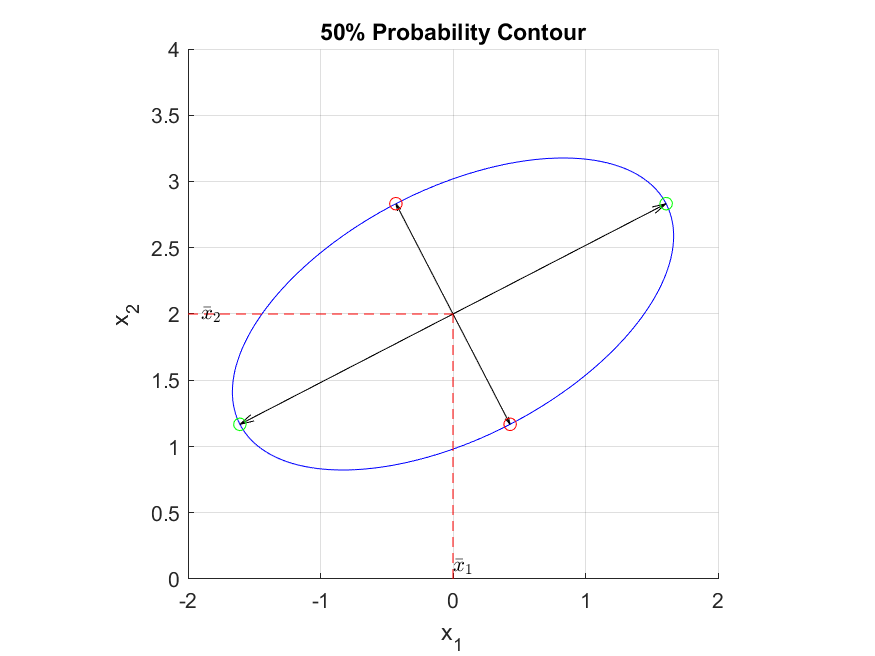
\includegraphics[scale=0.8]{./matlab/chapter-4/sol4.2.png}
\end{figure}
\end{enumerate}